\section{\system}


{\system} system is built to process articles,
provide fast response to user queries and display descriptive
results in a user interface.
In this section we describe our preprocessing steps to extract
topic models from the documents.
We then discuss the User Model behind each user search.
Finally we discuss our methods for topic-based search and exploration.



\subsection{Data pre-processing and topic learning}

Here we describe the main pre-processing steps we perform on a 
collection of articles for topic modeling and search. First, 
we tokenize articles with the help of the python 
Natural Language Toolkit (NLTK)~\footnote{\texttt{http://www.nltk.org/}} and a set of 
predefined regular expressions. Next, we standardize tokens by 
removing noise and stop-words. We use typical normalization 
techniques for word tokens such as \textsl{stemming}, in particular we use the popular Porter stemming algorithm~\cite{Porter1980} 
implementation in NLTK\@. 
After building a vocabulary of corpus words, each document is represented as a sparse ``bag of words''.
Last, we use the processed documents as input to the topic 
learning algorithm~\cite{hoffman2010online} which will in turn learn 
the latent topic structure of a corpus from the term co-occurrence 
frequencies of the corresponding documents. %Components of a learned 
%topic model includes the estimated corpus-level topics, $\beta_j^{*}$s, 
%and document-level topic mixtures, $\theta_d^{*}$s. As discussed, 
%$\beta_j^{*}$ is useful for our automatic detection of topics among  
%articles. Similarly, $\theta_d^{*}$ give an idea of the topicality 
%of a particular article given a topic. This is quite useful in 
%finding similar articles and grouping them together. In addition, 
%topic modeling is a type of dimensionality reduction technique that 
%enables us to work on the topic-space rather than on the 
%vocabulary-space.



\subsection{User Model}
When performing search, exploration and discovery over articles 
users may bring particular context to their search. Incorporating 
this information into the search process has been shown to be 
beneficial to users~\cite{DZSRWJ,MZPGSOL}. We develop a user model 
that encapsulates the users personal context and integrates it into 
their search task. 

This model is a distribution of weights for each identified topic in 
a corpus. Formally, given a set of topics $\beta_j^{*}$s the user 
model is defined as
$$
\mathcal{U} = \{u_0, \ldots, u_{K}\}
$$
where $u_j \in [0,1]$, $\sum_{j = 1}^K u_j = 1$, $K$ is the number 
of topics in the corpus.
We allow the user to interactively select the weights that correspond to
each topic learned over the corpus. This allows the users to change preferences with each query
for more desirable results.

\subsection{User Model Reweighted Keyword Search}
The user model is used to provide better feedback to
the user. After a \textsl{keyword-based filter}, the document results of the search 
are re-ranked by calculating the KL-divergence of each document and the
user model. Formally, given the set of result documents $\cal D$:

\begin{equation} \label{eq:KL}
KL(\mathcal{U}||\theta^*_{d}) = \sum_{j = 1}^K u_j \ln \frac{u_j}{\theta^*_{dj}}.
\end{equation}
where $d \in {\cal D}$ and $\theta^*_{d}$ is the topic proportion 
for document $d$ from the LDA model. 

%In the topic explorer, each topic row is color-coded like a heat 
%based map based on the similarity of the user model to that topic (see Figure~\ref{fig:topic_exploration}).

\subsection{Topic-Based Search}

Another method of search is to identify the topics of 
real interest, observing the most \textsl{informative terms} in 
the estimated topics. 
To identify informative terms in a topic we can sort vocabulary 
terms in the order of their term probabilities.
That is, each vector $\beta_j^{*}$ in the topic matrix is sorted.
  
In literature, researchers have proposed several other methods for 
finding informative terms~\cite{2012-termite} and evaluating topics 
\cite{mimno2011optimizing}. In this paper, we use a visualization 
scheme called \textsl{word cloud}~\cite{Davis2013}, to visualize the 
most probable words in a topic. For example, see Figure 
\ref{fig:topic-word-cloud} for the visualizing of a topic that is 
extracted from a corpus, which is built from a subset of Wikipedia 
articles under the category \textsl{Whales}. 
       
\begin{figure*}[htb]\centering 
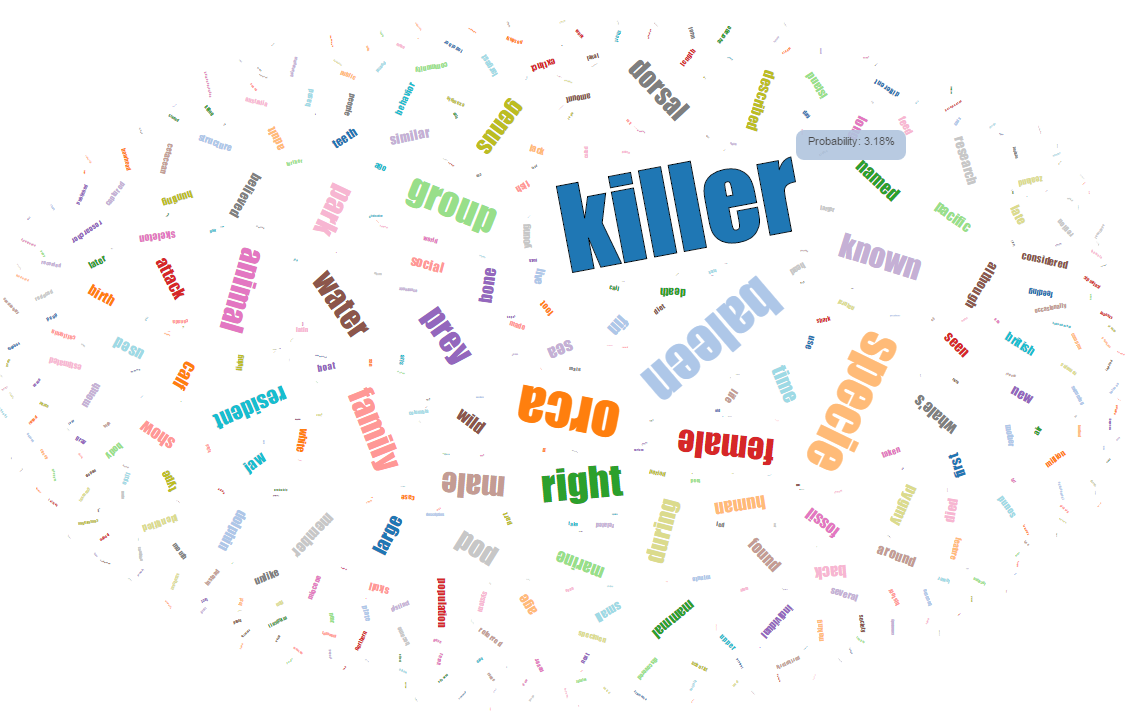
\includegraphics[width=.9\textwidth]{images/topic_visualization.png}
\caption{\textsl{Topic Word Cloud}. Words with high probabilities for the 
given topic are larger in size and words with low probabilities for 
the given topic are smaller in size. From the most probable words, 
we can infer that the topic mainly refers the Wikipedia category 
\textit{Killer Whales}---one of the main categories from which, we 
downloaded the articles for the corpus.}
\label{fig:topic-word-cloud}
\end{figure*}

We can exploit the estimated document specific topic distributions 
 of individual articles ($\theta_d^{*}$) in a corpus, to rank them on 
relevance for given a topic. Let $t$ be the index for the topic of 
interest. For each document $d = 1, 2, \ldots, D$ in the corpus, we 
can calculate~\cite{George2012}
\begin{equation}
m(d) = \ln \theta^*_{dt} + \sum_{j \neq t}{\ln (1 - \theta^*_{dj})},
\label{eq:topic-exploration}
\end{equation} 
where $j = 1, 2, \ldots, K$ and assume that each $\theta^*_{dt}$ is 
normalized, i.e., $\sum_{j=1}^{K}{\theta^*_{dj}} = 1$. We then sort 
the documents based on each $m(d)$ to rank them on relevance. 
Intuitively, we can see that Equation~\ref{eq:topic-exploration} 
will give a high value for a document, if the document is 
thematically related to the $t$th topic. 

\subsection{Topic-Based Exploration}

If a user find an interesting document and she would like to
find other similar documents she may use the topic-based method of exploration.
To visualize the hidden topical content of the article we use the 
estimated document topic distribution, $\theta^*_{d}$.
For example, Figure~\ref{fig:doc-topic-distribution} shows a Doughnut  
Chart\footnote{\texttt{https://developers.google.com/chart}} 
visualization for the Wikipedia article \textit{Killer Whale}.
It is an article listed under the Wikipedia category          
\textit{Killer Whales}. Different slices of the doughnut chart represent
different topics in the article \textit{Killer Whale}. The size 
of a slice represents the probability of a topic given the article. 
For this illustration, we labeled all the topic 
distributions obtained via the LDA posterior inference, on a 
corpus that is built using a subset of Wikipedia articles under the 
category \textit{Whales}. We used the topic word clouds 
and the Wikipedia subcategories under the category \textit{Whales} 
for labeling. Once we find an interesting topic to pursue, we can 
explore all the relevant documents under that topic using the 
method described in the previous section. 

\begin{figure}[htb]\centering 
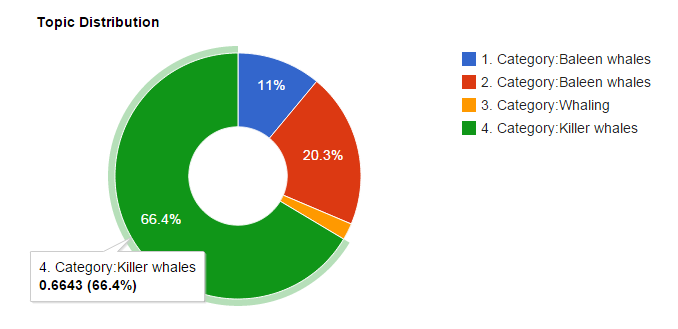
\includegraphics[width=.45\textwidth]{images/doc_topic_distribution.png}
\caption{Visualization of the document specific topic distribution 
for the Wikipedia article \textit{Killer Whale}.}
\label{fig:doc-topic-distribution}
\end{figure}

Another way to visualize a document is to look at its 
\textsl{paragraph} or \textsl{section} specific topic distributions. 
Each section or paragraph is written with careful attention is every 
peer review article or paper. While looking at an article or paper,  
one can easily identify which section or paragraph is of one's real 
interest. This intuition can be used to improve topic based 
exploration. We used the learned LDA model to 
estimate a section or paragraph's topic distribution using the
Gensim LDA implementation~\cite{rehurek_lrec}. This is an 
online task and is performed when a user selects a section or 
paragraph of an article, which is described in detail in the \system 
User Interface section.


Another interesting option to explore is how we can use an article's 
topic distribution for searching similar articles of interest. 
Recall that LDA enables us to transform documents in a corpus into 
vectors ($\theta^*_{d}$) in a lower dimensional topic space 
of that corpus. One can then define similarity between two documents 
via any typical vector space similarities, e.g., cosine similarity. 
%In \system we call this as article \textsl{lineage search}.         

